
\pagebreak
\section{La gestion de la qualité}

Le thème gestion de la qualité comporte deux domaines : 

\vspace{\baselineskip}

\begin{itemize}
\item
\textbf{Gestion de la qualité} : Une documentation existante (processus, directives, etc.) peut être intégrée dans CUBE PA.
\item
\textbf{Manuels} : Une documentation structurée (manuels de projet, etc.) peut être créée dans CUBE PA.
\end{itemize}

\vspace{\baselineskip}

\subsection{Gestion de la qualité}

Vous pouvez intégrer des documents existants dans CUBE PA pour les rendre accessibles à une équipe de projet. Veuillez noter que les liens aux documents peuvent uniquement être créés par un administrateur. Veuillez contacter votre administrateur CUPE PA ou envoyez un courriel au support CUBE PA : {\color{red} cube.support@emchberger.ch}.

\subsubsection{Retrouver des documents de gestion de la qualité}

Vous pouvez retrouver un document lié de la manière suivante :

\vspace{\baselineskip}

\begin{wrapfigure}[12]{l}{6.5cm}   % [x] Wie manche Zeile soll sich um die Grafik "brechen"
  \vspace{-35pt}      % Grundwert war 20; mit 30 schön oben beim Text ausgerichtet
  \begin{center}
    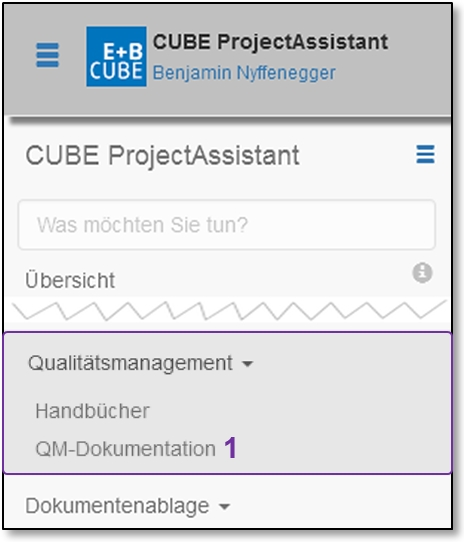
\includegraphics[width=1\linewidth]{../chapters/09_Qualitaetsmanagement/pictures/9-1_Menu_Qualitaetsmanagement.jpg}
  \end{center}
  \vspace{-20pt}
  \caption{Utiliser la gestion de la qualité}
  \vspace{-10pt}
\end{wrapfigure}

Dans le menu principal à gauche, sélectionnez l'élément de menu 'Gestion de la qualité' et dans cet exemple le sous-élément 'Documentation de gestion de la qualité' \col{(1)}. \\
 
\textbf{Remarque :} S'il existe des liens à plusieurs documents, ces derniers vont tous s'afficher comme sous-éléments sous l'élément de menu 'Gestion de la qualité'. Vous pouvez choisir les noms qui seront affichés (voir chapitre \ref{bkm:Ref912000789}). \\

\pagebreak

La vue suivante est maintenant affichée à droite :

\begin{figure}[H]
\center{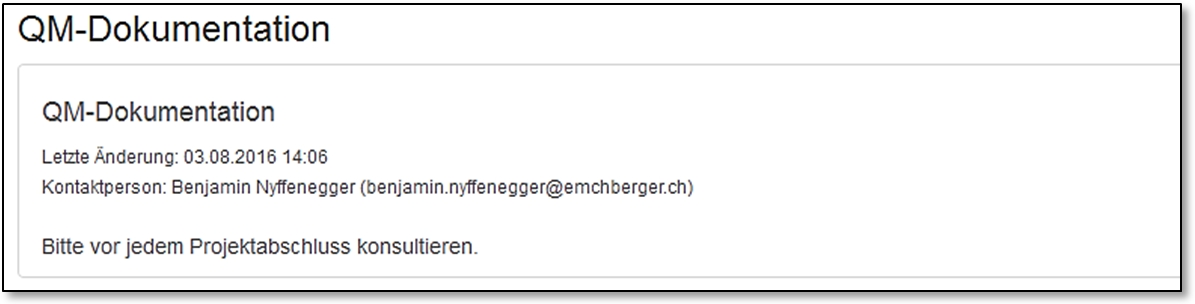
\includegraphics[width=1\linewidth]{../chapters/09_Qualitaetsmanagement/pictures/9-1_Verkn_Dokument.jpg}}
\caption{Ouvrir un document lié}
% \label{fig:speciation}
\end{figure}

Le nom du document et la description correspondante sont affichés. De plus, l'utilisateur responsable pour le document et la date de la dernière modification ou de chargement du document sont aussi indiqués. Cliquez sur les champs encadrés pour ouvrir le document ou pour le sauvegarder sur votre ordinateur. Une fenêtre de dialogue sera affichée ; son contenu dépend du navigateur que vous utilisez.

\subsubsection{Créer des liens à des documents dans la gestion de la qualité}
\label{bkm:Ref912000789}

Ce processus nécessite des droits d'accès spécifiques dans CUBE PA. Veuillez contacter votre administrateur CUBE PA ou envoyer un courriel au support CUBE PA : {\color{red} cube.support@emchberger.ch}.

\vspace{\baselineskip}

Pour lier un (ou plusieurs) document(s) à la 'Gestion de la qualité', procédez comme suit :

\vspace{\baselineskip}

\textbf{1ère étape : Créer des 'Types de données d'affichage'}

Dans un premier temps, une nouvelle désignation pour le menu doit être créée (dans notre exemple c'est la désignation 'Documentation de gestion de la qualité'). Pour ce faire, choisissez l'élément 'Configuration' dans le menu principal puis le sous-élément 'Types de données d'affichage'. L'aperçu de tous les types de données d'affichage existants s'affiche. Vous pouvez créer une nouvelle saisie en utilisant le symbole plus (ajouter) 
\includegraphics[height=12pt]{/Icons/Plussymbol.jpg} \col{(1)} :

\begin{figure}[H]
\center{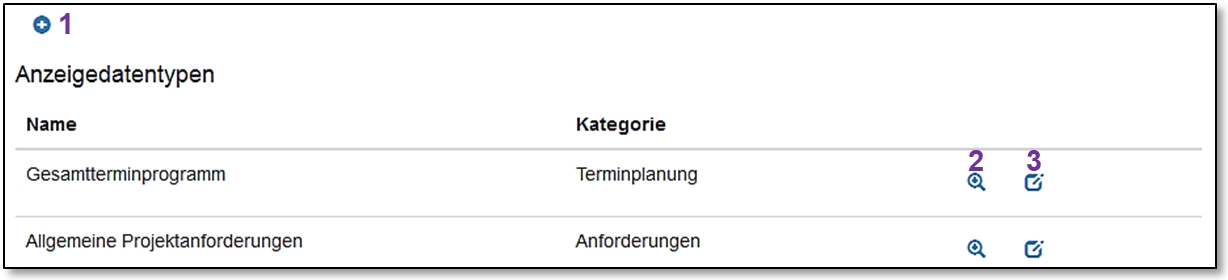
\includegraphics[width=1\linewidth]{../chapters/09_Qualitaetsmanagement/pictures/9-1-1_Anzeigedatentypen_Uebersicht.jpg}}
\caption{Aperçu des types de données d'affichage}
% \label{fig:speciation}
\end{figure}

Le symbole de loupe 
\includegraphics[height=12pt]{/Icons/Lupe.jpg} \col{(2)} vous permet d'afficher le contenu des saisies existantes. Le symbole de crayon 
\includegraphics[height=12pt]{/Icons/Bearbeiten.jpg} \col{(3)} vous permet de modifier une saisie existante. En cliquant sur le symbole plus (ajouter) 
\includegraphics[height=12pt]{/Icons/Plussymbol.jpg} \col{(1)} vous accédez aux informations et paramètres suivants :

\begin{figure}[H]
\center{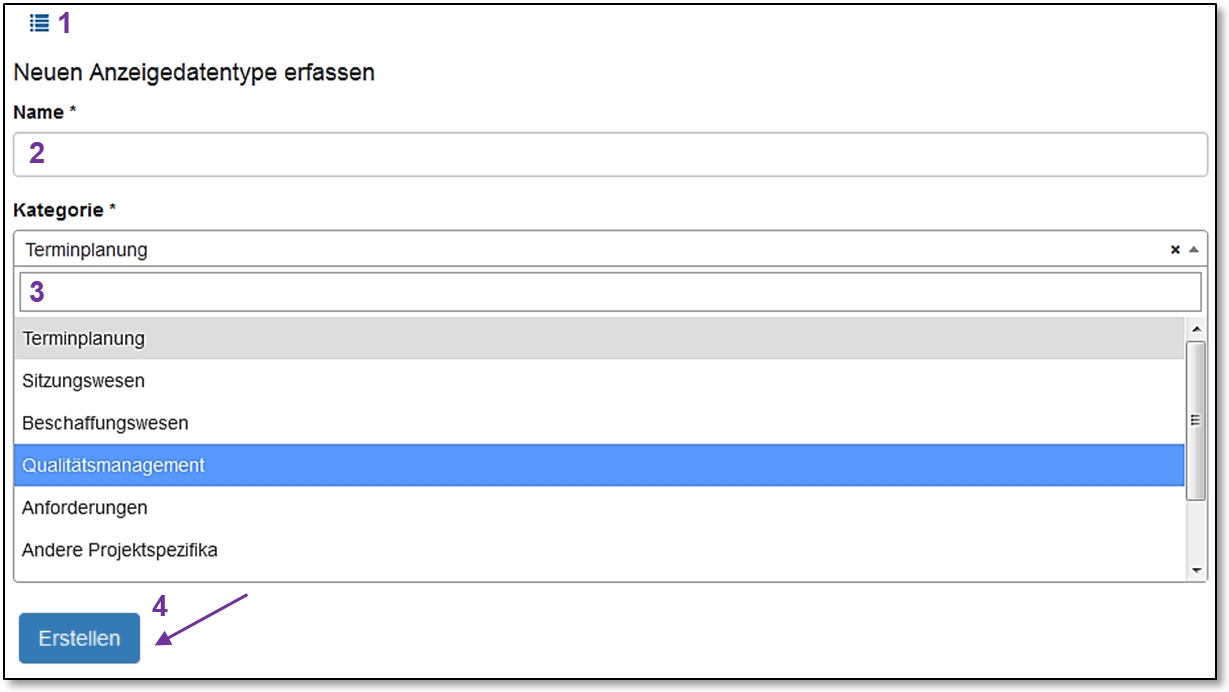
\includegraphics[width=1\linewidth]{../chapters/09_Qualitaetsmanagement/pictures/9-1-1_Anzeigedatentypen_Eingaben.jpg}}
\caption{Créer un type de données d'affichage}
% \label{fig:speciation}
\end{figure}

Le symbole de liste 
\includegraphics[height=12pt]{/Icons/Listensymbol_zurueck.jpg} \col{(1)} vous permet de retourner à l'aperçu. Saisissez le nom du lien au document \col{(2)} (ce nom apparaîtra dans le menu CUBE PA). Sous 'Catégorie' \col{(3)}, sélectionnez 'Gestion de la qualité' dans le menu déroulant et cliquez sur 'Créer'. Les données sont sauvegardées.

\vspace{\baselineskip}

\textbf{2ème étape : Créer des 'Données d'affichage'}

Pour créer la saisie qui contient le document lié, sélectionnez l'élément de menu 'Configuration' puis le sous-élément 'Données d'affichage'. L'aperçu suivant est affiché : 

\begin{figure}[H]
\center{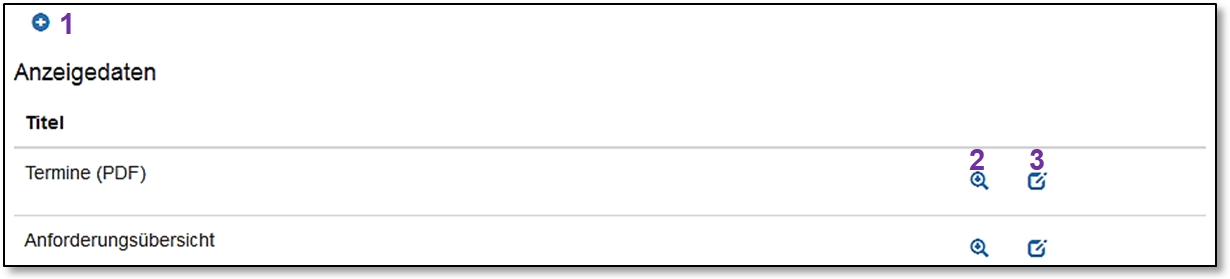
\includegraphics[width=1\linewidth]{../chapters/09_Qualitaetsmanagement/pictures/9-1-1_Anzeigedaten_Uebersicht.jpg}}
\caption{Aperçu des données d'affichage}
% \label{fig:speciation}
\end{figure}

Le symbole plus (ajouter) 
\includegraphics[height=12pt]{/Icons/Plussymbol.jpg} \col{(1)} vous permet de créer une nouvelle saisie. Le symbole de loupe 
\includegraphics[height=12pt]{/Icons/Lupe.jpg} \col{(2)} ou le symbole de crayon 
\includegraphics[height=12pt]{/Icons/Bearbeiten.jpg} \col{(3)} vous permettent d'afficher ou de modifier une saisie existante, respectivement. Cliquez sur le symbole plus (ajouter) 
\includegraphics[height=12pt]{/Icons/Plussymbol.jpg} \col{(1)} pour créer un nouveau lien à un document.

\begin{figure}[H]
\center{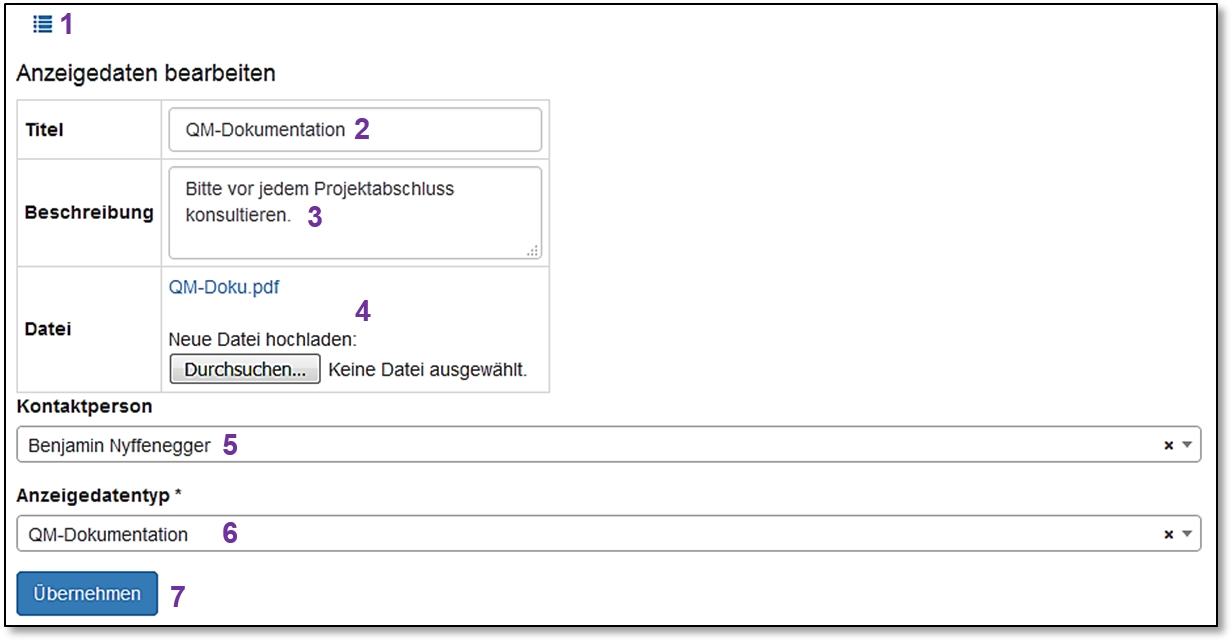
\includegraphics[width=1\linewidth]{../chapters/09_Qualitaetsmanagement/pictures/9-1-1_Anzeigedaten_Eingaben.jpg}}
\caption{Créer une donnée d'affichage}
% \label{fig:speciation}
\end{figure}

Le symbole de liste 
\includegraphics[height=12pt]{/Icons/Listensymbol_zurueck.jpg} \col{(1)} vous permet de retourner à l'aperçu. Saisissez le titre désiré \col{(2)} (au mieux le même que le titre saisi sous 'Types de données d'affichage'). Vous pouvez ajouter une description \col{(2)}, qui sera ensuite affichée sous 'Gestion de la qualité' et l'élément de menu correspondant / créé. Sous 'Fichier' \col{(4)} vous pouvez charger et lier le document désiré. Cliquez sur 'Parcourir' et choisissez ensuite le document désiré dans la fenêtre Explorer.\\

Vous pouvez optionnellement choisir une personne de contact \col{(5)}. Son nom sera affiché et son adresse e-mail enregistrée. Sélectionnez le type de données d'affichage auquel cette donnée d'affichage doit être liée \col{(6)}. Cliquez sur 'Accepter' pour sauvegarder les données. Le document lié peut maintenant être ouvert à travers l'élément de menu 'Gestion de la qualité' et le sous-élément correspondant. Voici un aperçu commenté de la saisie du document, afin de mieux expliquer quelles données sont affichées :

\begin{figure}[H]
\center{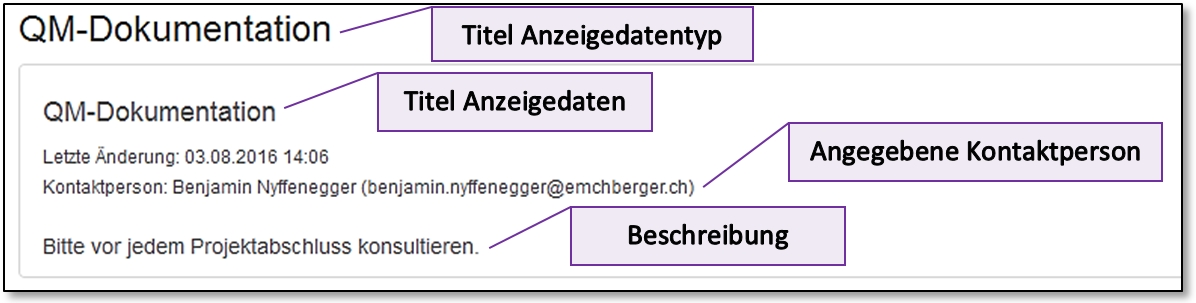
\includegraphics[width=1\linewidth]{../chapters/09_Qualitaetsmanagement/pictures/9-1-1_AngezeigteDaten.jpg}}
\caption{Types de données d'affichage sous la gestion de la qualité}
% \label{fig:speciation}
\end{figure}

Si le document lié est modifié, vous pouvez modifier la saisie existante et simplement charger le nouveau document. Le champ 'Dernière mise à jour' sera actualisé en conséquence et le nouveau document sera disponible.

\subsection{Manuel de projet}

\begin{wrapfigure}[6]{l}{6.5cm}   % [x] Wie manche Zeile soll sich um die Grafik "brechen"
  \vspace{-35pt}      % Grundwert war 20; mit 30 schön oben beim Text ausgerichtet
  \begin{center}
    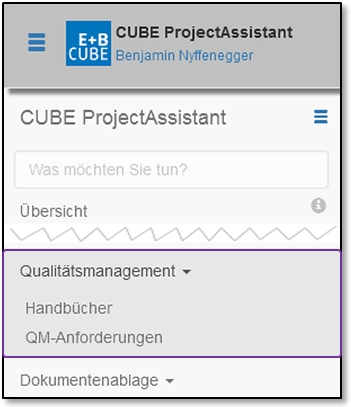
\includegraphics[width=1\linewidth]{../chapters/09_Qualitaetsmanagement/pictures/9-2_Menu_Qualitaetsmanagement_Handbuch.jpg}
  \end{center}
  \vspace{-20pt}
  \caption{La fonction manuel dans CUBE PA}
  \vspace{-10pt}
\end{wrapfigure}

Sous la gestion de la qualité, vous pouvez élaborer des manuels, comme par exemple un manuel de projet. Pour ce faire, sélectionnez l'élément de menu 'Gestion de la qualité' puis le sous-élément 'Manuels'.

\vspace{2.5cm} 

Si vous avez déjà ajouté des manuels, ces derniers seront disponibles dans l'aperçu : \\

\vspace{3cm}  

\begin{figure}[H]
\center{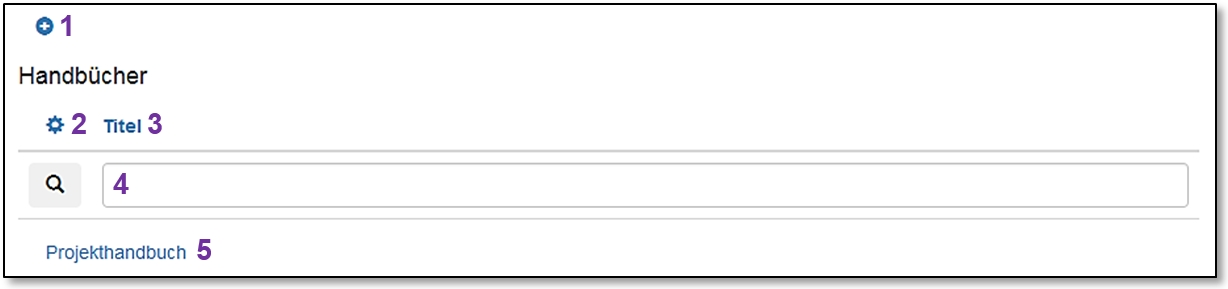
\includegraphics[width=1\linewidth]{../chapters/09_Qualitaetsmanagement/pictures/9-2_Handbuch_Uebersicht.jpg}}
\caption{Aperçu des manuels}
% \label{fig:speciation}
\end{figure}

Le symbole plus (ajouter) 
\includegraphics[height=12pt]{/Icons/Plussymbol.jpg} \col{(1)} vous permet d'ajouter un manuel supplémentaire (voir chapitre \ref{bkm:Ref930000788}). Le symbole de configuration 
\includegraphics[height=12pt]{/Icons/SpaltenEinst.jpg} \col{(2)} vous permet d'afficher ou de masquer des colonnes (ceci n'a pas d'effet dans l'aperçu des manuels puisqu'il n'y a qu'une seule colonne). Cliquez sur l'en-tête bleu \col{(3)} pour classer les manuels affichés par ordre alphabétique croissant ou décroissant. Si vous cherchez un manuel en particulier, saisissez un terme dans le champ de recherche \col{(4)} puis cliquez sur le symbole de loupe 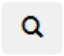
\includegraphics[height=12pt]{/Icons/Lupe_s.jpg} ou appuyez la touche Entrée. La liste filtrée de documents / manuels s'affiche. (Attention : Le filtre permet de chercher uniquement dans les titres des manuels et pas dans leur contenu). Cliquez sur un manuel \col{(5)} pour l'ouvrir :

\begin{figure}[H]
\center{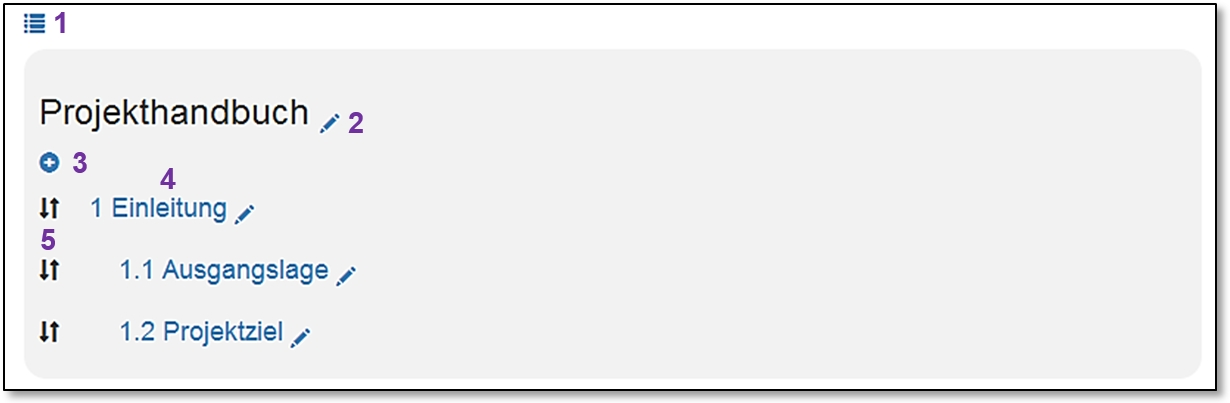
\includegraphics[width=.75\linewidth]{../chapters/09_Qualitaetsmanagement/pictures/9-2_Projekthandbuch.jpg}}
\caption{Aperçu d'un manuel}
% \label{fig:speciation}
\end{figure}

Le symbole de liste 
\includegraphics[height=12pt]{/Icons/Listensymbol_zurueck.jpg} \col{(1)} vous permet de retourner à l'aperçu. Le manuel apparaît alors dans l'aperçu. Le symbole de crayon 
\includegraphics[height=12pt]{/Icons/Stift.jpg} \col{(2)} vous permet de modifier la saisie et le symbole plus (ajouter) 
\includegraphics[height=12pt]{/Icons/Plussymbol.jpg} \col{(3)} vous permet d'ajouter un nouveau chapitre. Lorsque vous cliquez sur le titre d'un chapitre (en bleu) \col{(4)}, ce chapitre est ouvert. Pour modifier la position d'un chapitre, glissez le symbole de flèches verticales 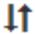
\includegraphics[height=12pt]{/Icons/VertPfeile.jpg} \col{(5)} à côté du chapitre et déposez-le à la position voulue. \\
Vous pouvez sauvegarder le manuel en entier sous forme PDF. Pour ce faire, cliquez sur le symbole de téléchargement 
\includegraphics[height=12pt]{/Icons/Download.jpg} \col{(6)}. Un fichier zip contenant le manuel sous forme PDF et tout document associé est téléchargé.

\subsubsection{Modifier un manuel existant}

Le titre d'un manuel peut directement être modifié dans l'aperçu (en cliquant sur le symbole de crayon 
\includegraphics[height=12pt]{/Icons/Stift.jpg} \col{(2)}). Après la modification, cliquez sur la coche sous le titre. La modification est enregistrée :

\begin{figure}[H]
\center{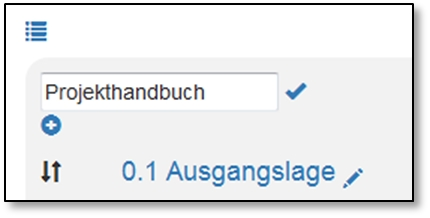
\includegraphics[width=0.35\linewidth]{../chapters/09_Qualitaetsmanagement/pictures/9-2-1_HandbuchTitel_aendern.jpg}}
\caption{Modifier le titre d'un manuel}
% \label{fig:speciation}
\end{figure}

Pour modifier une saisie, cliquez sur le symbole de crayon 
\includegraphics[height=12pt]{/Icons/Stift.jpg} à côté du chapitre désiré. Le masque de saisie suivant s'affiche :

\begin{figure}[H]
\center{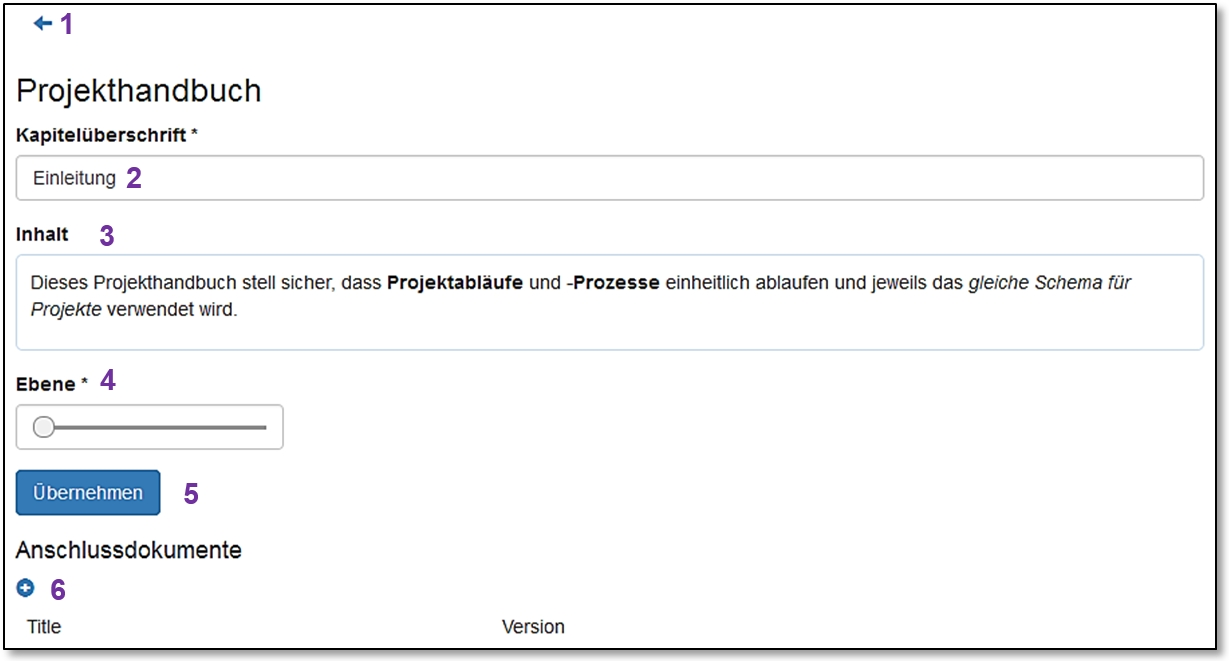
\includegraphics[width=1\linewidth]{../chapters/09_Qualitaetsmanagement/pictures/9-2-1_Handbuch_aendern.jpg}}
\caption{Modifier un chapitre}
% \label{fig:speciation}
\end{figure}

Cliquez sur le symbole de flèche pour retourner au manuel (aperçu) 
\includegraphics[height=12pt]{/Icons/Pfeil-links.jpg} \col{(1)}. Les saisies existantes peuvent être modifiées dans les différents champs de saisie. Vous pouvez modifier le titre d'un chapitre \col{(2)} (le titre d'un chapitre est un champ obligatoire et doit être / rester rempli). Vous pouvez modifier le contenu \col{(3)} d'un chapitre. Le régulateur de niveau \col{(4)} vous permet de modifier la hiérarchie des chapitres. Déplacez le curseur à gauche pour mettre un chapitre au premier niveau (1), au milieu pour le mettre au premier niveau inférieur (1.1), et à droite pour le mettre au deuxième niveau inférieur (1.1.1). \\

Des documents peuvent être liés à des chapitres spécifiques. Le symbole plus 
\includegraphics[height=12pt]{/Icons/Plussymbol.jpg} \col{(6)} offre un aperçu des documents liés :

\begin{figure}[H]
\center{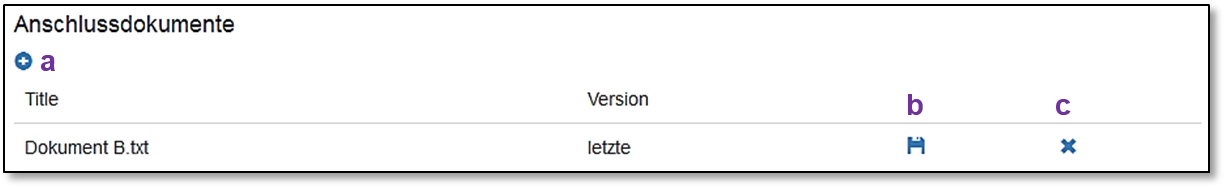
\includegraphics[width=1\linewidth]{../chapters/09_Qualitaetsmanagement/pictures/9-2-1_Anschlussdokumente_aendern.jpg}}
\caption{Documents liés}
% \label{fig:speciation}
\end{figure}

Vous pouvez ajouter un document en cliquant sur le symbole plus (ajouter) 
\includegraphics[height=12pt]{/Icons/Plussymbol.jpg} \col{(a)}. Vous pouvez enregistrer un document existant sur votre ordinateur en cliquant le symbole d'enregistrement 
\includegraphics[height=12pt]{/Icons/Diskette.jpg} \col{(b)} ou le supprimer en cliquant sur la croix 
\includegraphics[height=12pt]{/Icons/Kreuzchen.jpg} \col{(c)}.

Cliquez sur 'Accepter' \col{(5)} pour enregistrer les modifications. 

\subsubsection{Créer un nouveau manuel}
\label{bkm:Ref930000788}

Procédez comme suit pour créer un nouveau manuel :

Dans le menu principal, choisissez l'élément 'Gestion de la qualité' et le sous-élément 'Manuels'. Dans l'aperçu des manuels, cliquez sur le symbole plus (ajouter) 
\includegraphics[height=12pt]{/Icons/Plussymbol.jpg} \col{(1)}.

\begin{figure}[H]
\center{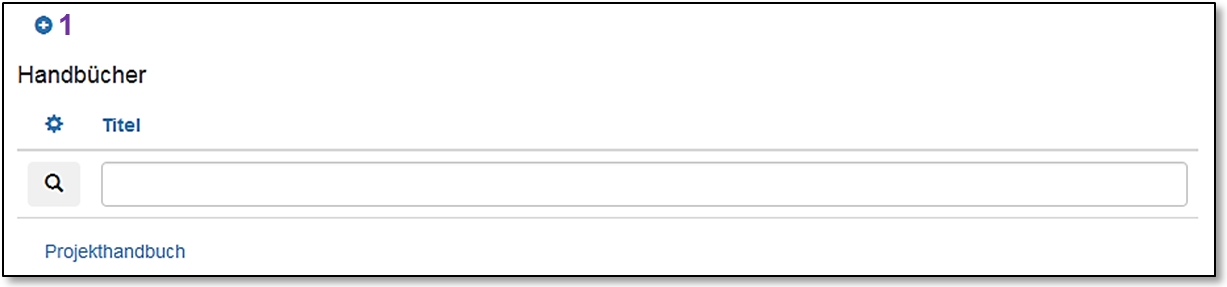
\includegraphics[width=1\linewidth]{../chapters/09_Qualitaetsmanagement/pictures/9-3-2_NeuesHandbuch_erstellen.jpg}}
\caption{Créer un nouveau manuel}
% \label{fig:speciation}
\end{figure}

Saisissez un titre pour le nouveau manuel :

\begin{figure}[H]
\center{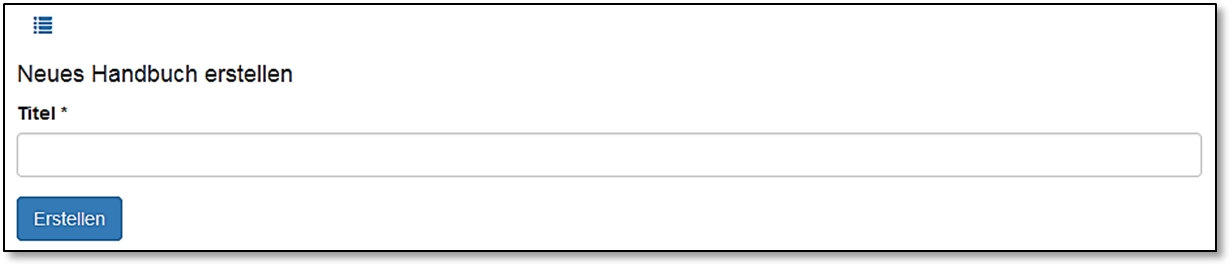
\includegraphics[width=1\linewidth]{../chapters/09_Qualitaetsmanagement/pictures/9-3-2_Handbuch_erstellen_Titel.jpg}}
\caption{Créer un nouveau manuel - Saisir un titre}
% \label{fig:speciation}
\end{figure}

Cliquez ensuite sur le bouton 'Créer'. Le manuel est créé.

\begin{figure}[H]
\center{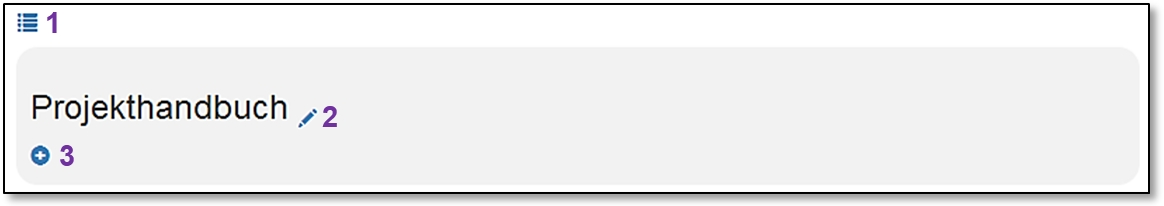
\includegraphics[width=.8\linewidth]{../chapters/09_Qualitaetsmanagement/pictures/9-3-2_Handbuch_angelegt.jpg}}
\caption{Nouveau manuel - Ajouter un chapitre}
% \label{fig:speciation}
\end{figure}

Le symbole de liste 
\includegraphics[height=12pt]{/Icons/Listensymbol_zurueck.jpg} \col{(1)} vous permet de retourner à l'aperçu des manuels. Le symbole de crayon 
\includegraphics[height=12pt]{/Icons/Stift.jpg} \col{(2)} vous permet de modifier le titre du manuel. Le symbole plus (ajouter) 
\includegraphics[height=12pt]{/Icons/Plussymbol.jpg} \col{(3)} vous permet d'ajouter des chapitres :

\begin{figure}[H]
\center{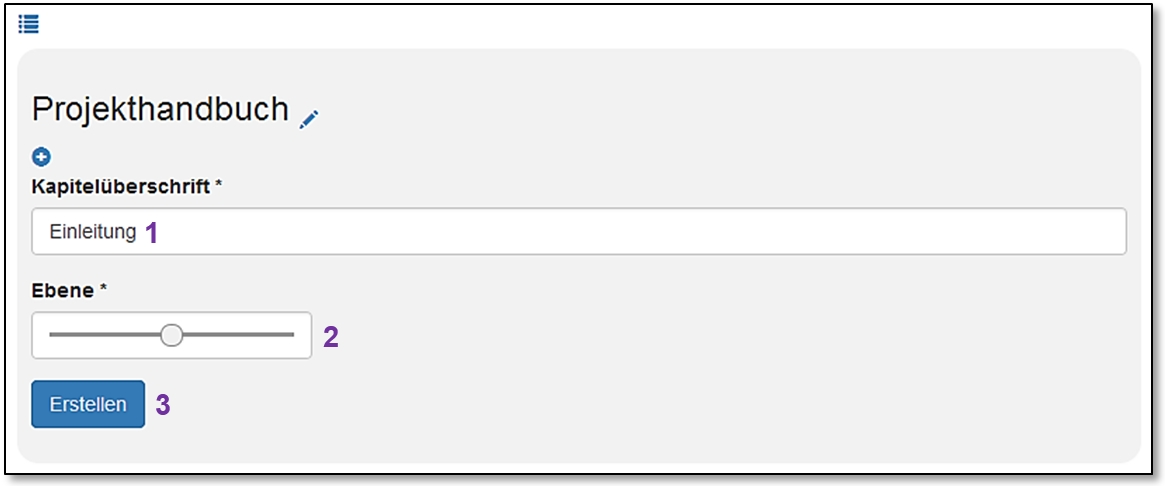
\includegraphics[width=.8\linewidth]{../chapters/09_Qualitaetsmanagement/pictures/9-3-2_Kapitel_anlegen.jpg}}
\caption{Nouveau manuel - Saisir le titre d'un chapitre}
% \label{fig:speciation}
\end{figure}

Saisissez le titre désiré du chapitre \col{(1)}. Vous avez déjà la possibilité de fixer le niveau du chapitre (gauche : 1, milieu : 1.1, droite : 1.1.1) \col{(2)}. Vous pouvez modifier le niveau du chapitre à un stade ultérieur. Cliquez ensuite sur 'Créer'. Le chapitre est créé et le masque de saisie change :

\begin{figure}[H]
\center{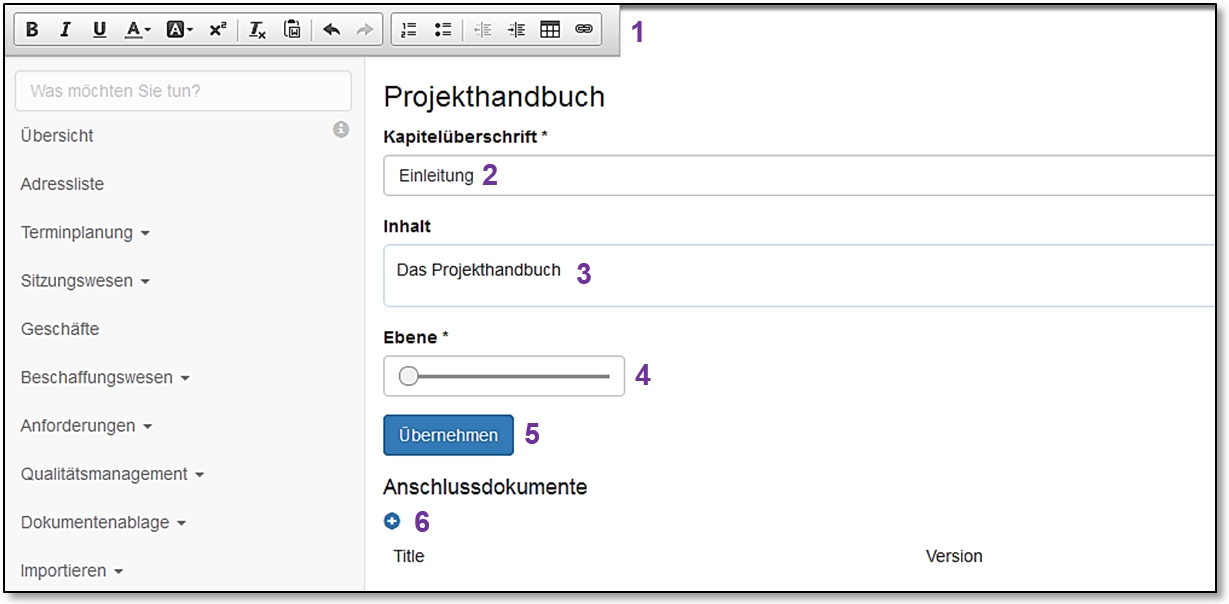
\includegraphics[width=1\linewidth]{../chapters/09_Qualitaetsmanagement/pictures/9-2-3_Kapitel_bearbeiten.jpg}}
\caption{Nouveau manuel - Modifier un chapitre}
% \label{fig:speciation}
\end{figure}

Vous pouvez toujours modifier le titre du chapitre \col{(2)}. Lorsque vous cliquez sur le champ 'Contenu' \col{(3)}, un menu s'affiche en haut à gauche \col{(1)}. Ce menu vous permet de formater le texte, de créer des tableaux, ou d'annuler des modifications (voir plus bas pour plus de détails). Vous pouvez également modifier le niveau du chapitre avec le régulateur de niveau \col{(4)}. Les changements sont enregistrés en cliquant le bouton 'Accepter' \col{(5)}. Une fonction additionnelle devient disponible : vous pouvez ajouter des documents ou des liens au chapitre \col{(6)}. Pour ce faire, cliquez sur le symbole plus (ajouter) 
\includegraphics[height=12pt]{/Icons/Plussymbol.jpg} \col{(6)}.

\begin{figure}[H]
\center{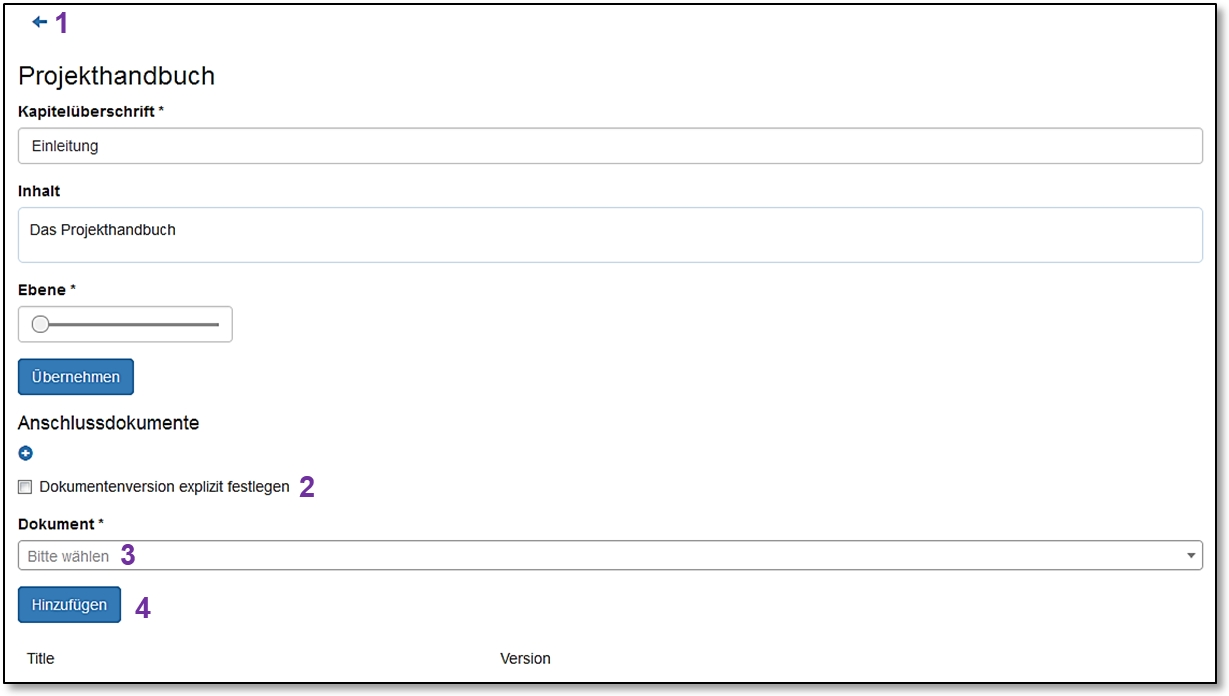
\includegraphics[width=1\linewidth]{../chapters/09_Qualitaetsmanagement/pictures/9-3-2_Kapitel_Dokumente_hinzufuegen.jpg}}
\caption{Nouveau manuel - Ajouter des documents}
% \label{fig:speciation}
\end{figure}

En créant ou modifiant un manuel, vous pouvez retourner à l'aperçu du manuel en cliquant sur le symbole de flèche 
\includegraphics[height=12pt]{/Icons/Pfeil-links.jpg} \col{(1)}. Par contre, les modifications que vous auriez faites seront perdues si vous ne cliquez pas d'abord sur le bouton 'Accepter'. Si vous vous trouvez dans le champ 'Contenu', le symbole de flèche sera caché. Cliquez dans un autre champ, par exemple dans le champ du titre du chapitre pour rendre le symbole de flèche visible. \\

\textbf{Lier des documents :} En bas de la fenêtre, vous pouvez choisir un document et le lier au chapitre. Tous les documents chargés sur CUBE PA dans le classement des documents sont disponibles dans la sélection. Si vous souhaitez faire un lien à un nouveau document pendant que vous travaillez sur un manuel, enregistrer vos modifications en cliquant sur le bouton 'Accepter' puis chargez le document souhaité dans la section 'Classement des documents'. Le chapitre \ref{bkm:Ref442863508} offre plus d'informations sur le chargement de documents. \\

La fonction 'Fixer la version du document' \col{(2)} vous permet de créer le lien vers une version spécifique d'un document. Si vous n'utilisez pas cette fonction, c'est la version la plus récente du document trouvée dans le classement des documents qui sera liée au chapitre. Dans certaines situations, il est nécessaire qu'une version spécifique d'un document soit liée. Pour ce faire, cochez la case pour activer la fonction. Vous trouverez plus d'informations par rapport à la gestion de documents et aux versions d'un document au chapitre \ref{bkm:Ref443047930}. \\

Répétez les étapes précédentes pour lier des documents additionnels. \\

\textbf{Formatage de texte et autres fonctions :}

\begin{figure}[H]
\center{\includegraphics[width=.8\linewidth]{../chapters/09_Qualitaetsmanagement/pictures/9-2-3_Text_formatieren.jpg}}
\caption{Nouveau manuel - Formatage de texte}
% \label{fig:speciation}
\end{figure}

Le contenu d'un chapitre peut être modifié, des tableaux peuvent être ajoutés, et des liens vers des sites web peuvent être créés comme dans un logiciel de traitement de texte. Voici un aperçu des différentes fonctions disponibles : \\

\begin{tabular}{c | p{14cm} l} %{cl}
\hline
\includegraphics[height=12pt]{../chapters/09_Qualitaetsmanagement/pictures/Format/Fett.jpg} & Le texte sera affiché en caractères gras \\
\hline
\includegraphics[height=12pt]{../chapters/09_Qualitaetsmanagement/pictures/Format/Kursiv.jpg} & Le texte sera affiché en italique \\
\hline
\includegraphics[height=12pt]{../chapters/09_Qualitaetsmanagement/pictures/Format/Unterstrichen.jpg} & Le texte sera souligné \\
\hline
\includegraphics[height=12pt]{../chapters/09_Qualitaetsmanagement/pictures/Format/Textfarbe.jpg} & La couleur du texte peut être modifiée \\
\hline
\includegraphics[height=12pt]{../chapters/09_Qualitaetsmanagement/pictures/Format/Hintergrundfarbe.jpg} & La couleur de fond du texte peut être modifiée \\
\hline
\includegraphics[height=12pt]{../chapters/09_Qualitaetsmanagement/pictures/Format/Form_z.jpg} & Le formatage de texte sera supprimé \\
\hline
\includegraphics[height=12pt]{../chapters/09_Qualitaetsmanagement/pictures/Format/ausWord.jpg} & Du contenu situé dans le clipboard, par exemple en provenance de Word, peut être ajouté. (Un message apparaît si le navigateur ne supporte pas cette fonction. Par contre, vous pouvez toujours coller le texte copié dans le champ qui apparaît et le transférer à CUBE PA.) \\
\hline
\includegraphics[height=12pt]{../chapters/09_Qualitaetsmanagement/pictures/Format/Undo.jpg} & Ces boutons vous permettent d'annuler ou de rétablir votre dernière modification \\
\hline
\includegraphics[height=12pt]{../chapters/09_Qualitaetsmanagement/pictures/Format/Aufzaehlung.jpg} & Le texte est converti en liste numérotée ou avec des points d'énumération  \\
\hline
\includegraphics[height=12pt]{../chapters/09_Qualitaetsmanagement/pictures/Format/Einruecken.jpg} & L'alinéa est réduit (texte déplacé à gauche) ou augmenté (texte déplacé à droite) \\
\hline
\includegraphics[height=12pt]{../chapters/09_Qualitaetsmanagement/pictures/Format/Tabellen.jpg} & Un tableau est inséré. Les tableaux peuvent être légendés et formatés (bordures, taille, direction, etc.) \\
\hline
\includegraphics[height=12pt]{../chapters/09_Qualitaetsmanagement/pictures/Format/Link.jpg} & Des liens à des sites web ou des références au sein du manuel peuvent être ajoutés. Des adresses e-mail peuvent aussi être inclues dans le manuel. \\
\hline
\end{tabular}

% bishierher




